We describe the choices we did about representation of the data and communication between modules.
These choices are described precisely in the documentation\footnote{\url{https://github.com/ProjetPP/Documentation/}} of the project.

\section{Data model}
\label{rdf}

First, we present the data model. All normalised structures of the PPP are JSON-serializable, i.e. they are trees made of instances of the following types:
\begin{itemize}
    \item \texttt{Object}
    \item \texttt{List}
    \item \texttt{String}
    \item \texttt{Number}
    \item \texttt{Boolean}
    \item \texttt{Null}
\end{itemize}

We chose to represent all normalised data as trees. To represent sentences, we have 4 kinds of nodes.

\begin{itemize}
    \item \texttt{sentence}: a question in natural language like "Who is George Washington?".
    \item \texttt{resource}: a leaf containing any kind of data (string, integer\ldots).
    \item \texttt{missing}: a leaf which marks missing values.
    \item \texttt{triple}: a 3-ary node:
        \begin{itemize}
            \item \texttt{subject}: what the triple refers to
            \item \texttt{predicate}: denotes the relationship between the subject and the
  object
            \item \texttt{object}: what property of the subject the triple refers to
        \end{itemize}         
\end{itemize}

For example, the work of the question parsing module is to transform 
\begin{verbatim}
{
    "type": "sentence", 
    "value": "Who is George Washington?"
}
\end{verbatim}
into 
\begin{verbatim}
{
    "type":
        "triple",
    "subject":{
        "type": "resource",
        "value": "George Washington"
    },
    "predicate":{
        "type": "resource",
        "value": "identity"
    },
    "object":{
        "type": "missing"
    }
}
\end{verbatim}

This structure has been chosen for its good adaptability. For instance, we can add other kind of nodes such as intersection, union, node for yes/no questions (triples without missing son), boolean operations, etc.

We do not plot explicitly the tree in the user interface, but we used a string representation defined recursively by:
\begin{itemize}
 \item A missing node is symbolized by a "\texttt{?}", possibly followed by an id (an integer).
 \item A resource word is symbolized by the corresponding string.
 \item A triple node of subject \texttt{subj}, predicate \texttt{pred} and object \texttt{obj} is symbolized by \texttt{(SUBJ,PRED,OBJ)} (where \texttt{SUBJ},  \texttt{PRED} and \texttt{OBJ} are the string representations of \texttt{subj}, \texttt{pred} and \texttt{obj}).
\end{itemize}

For instance, the previous tree will be represented by the string:

\begin{center}
    \texttt{(George Washington, identity, ?)}
\end{center}

\section{Communication}

Modules communicate with the core via HTTP requests.

The core sends them a JSON object, and they return another one.

The basic idea is that the core iterates requests to modules, which return a simplified tree, until the core gets a complete response, ie. a tree without any `missing` node.

During these exchanges, we keep a trace of the different steps between the original request and the current tree. The structure of a trace is a list of such trace items:
\begin{verbatim}
{
    "module":
        "<name of the module>", 
    "tree":{
        <answer tree>
    },
    "measures":{
        "relevance": <relevance of the answer>,
        "accuracy": <accuracy of the answer>
    }
}
\end{verbatim}

The measure field contains two values: relevance and accuracy.

\begin{itemize}
    \item \texttt{accuracy} is a self-rating of how much the module may have correctly understood (ie. not misinterpreted) the request/question. It is a float between 0 and 1.
    \item \texttt{relevance} is a self-rating of how much the tree has been improved (i.e. progressed on the path of becoming a useful answer). A positive float (not necessarily greater that 1; another module might use it to provide a much better answer).
\end{itemize}

This form allows each module to access to the previous results, particularly to the request of the user. The objects for request and response contain some extra data, such as the language used.

The data model have been implemented in a nice set of objects in both Python\footnote{\url{http://github.com/ProjetPP/PPP-datamodel-Python/}} and PHP\footnote{\url{http://github.com/ProjetPP/PPP-datamodel-PHP/}} in order to help the writing of modules.

We could define a linear representation for the trace, using the representation of the datamodel, but it is not relevant. Indeed, this information will never be printed on the user interface.

\begin{figure}[!ht]
% https://docs.google.com/drawings/d/1toUH24GqwtpvKV7S5gje6GBxfa13R3mxgm8WlAFc_0g/edit?usp=sharing
  \centering
    \label{datamodel:struct}
    \caption{Architecture of the PPP}
    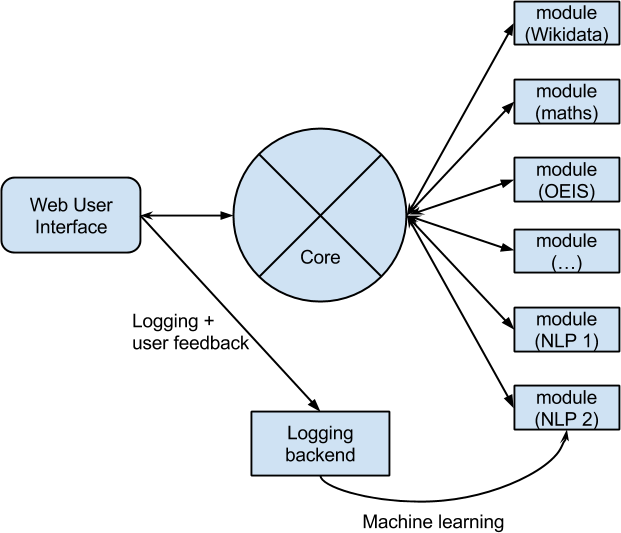
\includegraphics[width=0.8\textwidth]{../ppp_structure.png}
\end{figure}
